\section{Bối cảnh}
\headindent Hiện nay, Anime là một phần không thể thiếu của ngành công nghiệp giải trí Nhật Bản nói chung và thế giới nói riêng, với doanh thu hàng tỷ đô la mỗi năm. Cùng với sự phát triển của công nghệ, Anime đã không ngừng đổi mới, mang đến cho người xem những trải nghiệm độc đáo, phong phú về nội dung lẫn hình thức.

\vspace{1cm}
\begin{figure}[H]
\centerline{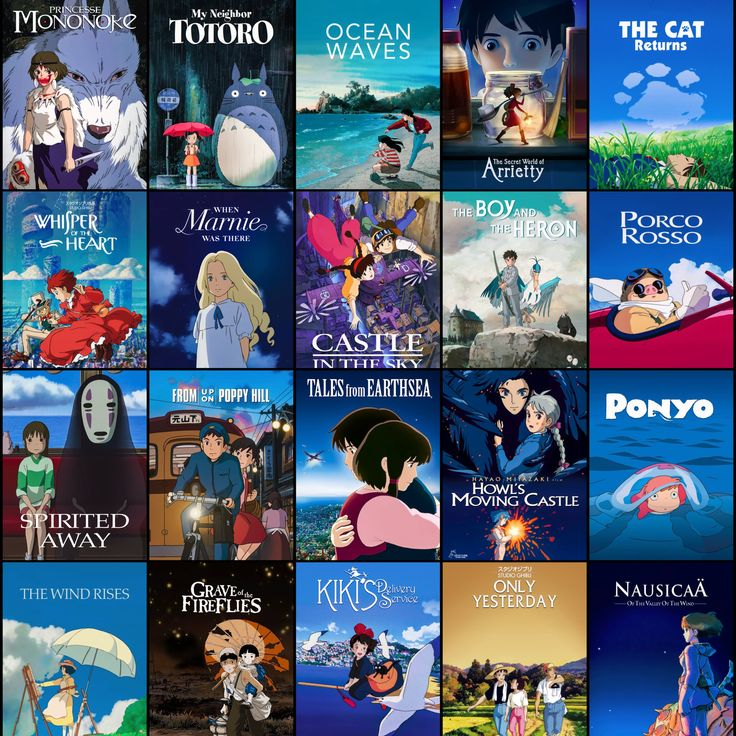
\includegraphics[width=\linewidth, height=0.8\linewidth]{content/background/image/studio.jpg}}
\caption{Studio Ghibli}
\label{fig}
\end{figure}
\pagebreak
\headindent Tại Việt Nam, hình thức giải trí này đang phát triển mạnh mẽ và trở thành một phần quan trọng trong văn hóa giải trí của giới trẻ:
\begin{itemize}
    \item Cộng đồng yêu thích anime ngày càng lớn, hoạt động sôi nổi trên mạng xã hội và các sự kiện offline, tạo nên một không gian gắn kết cho những người có chung sở thích.
    \begin{figure}[H]
    \centerline{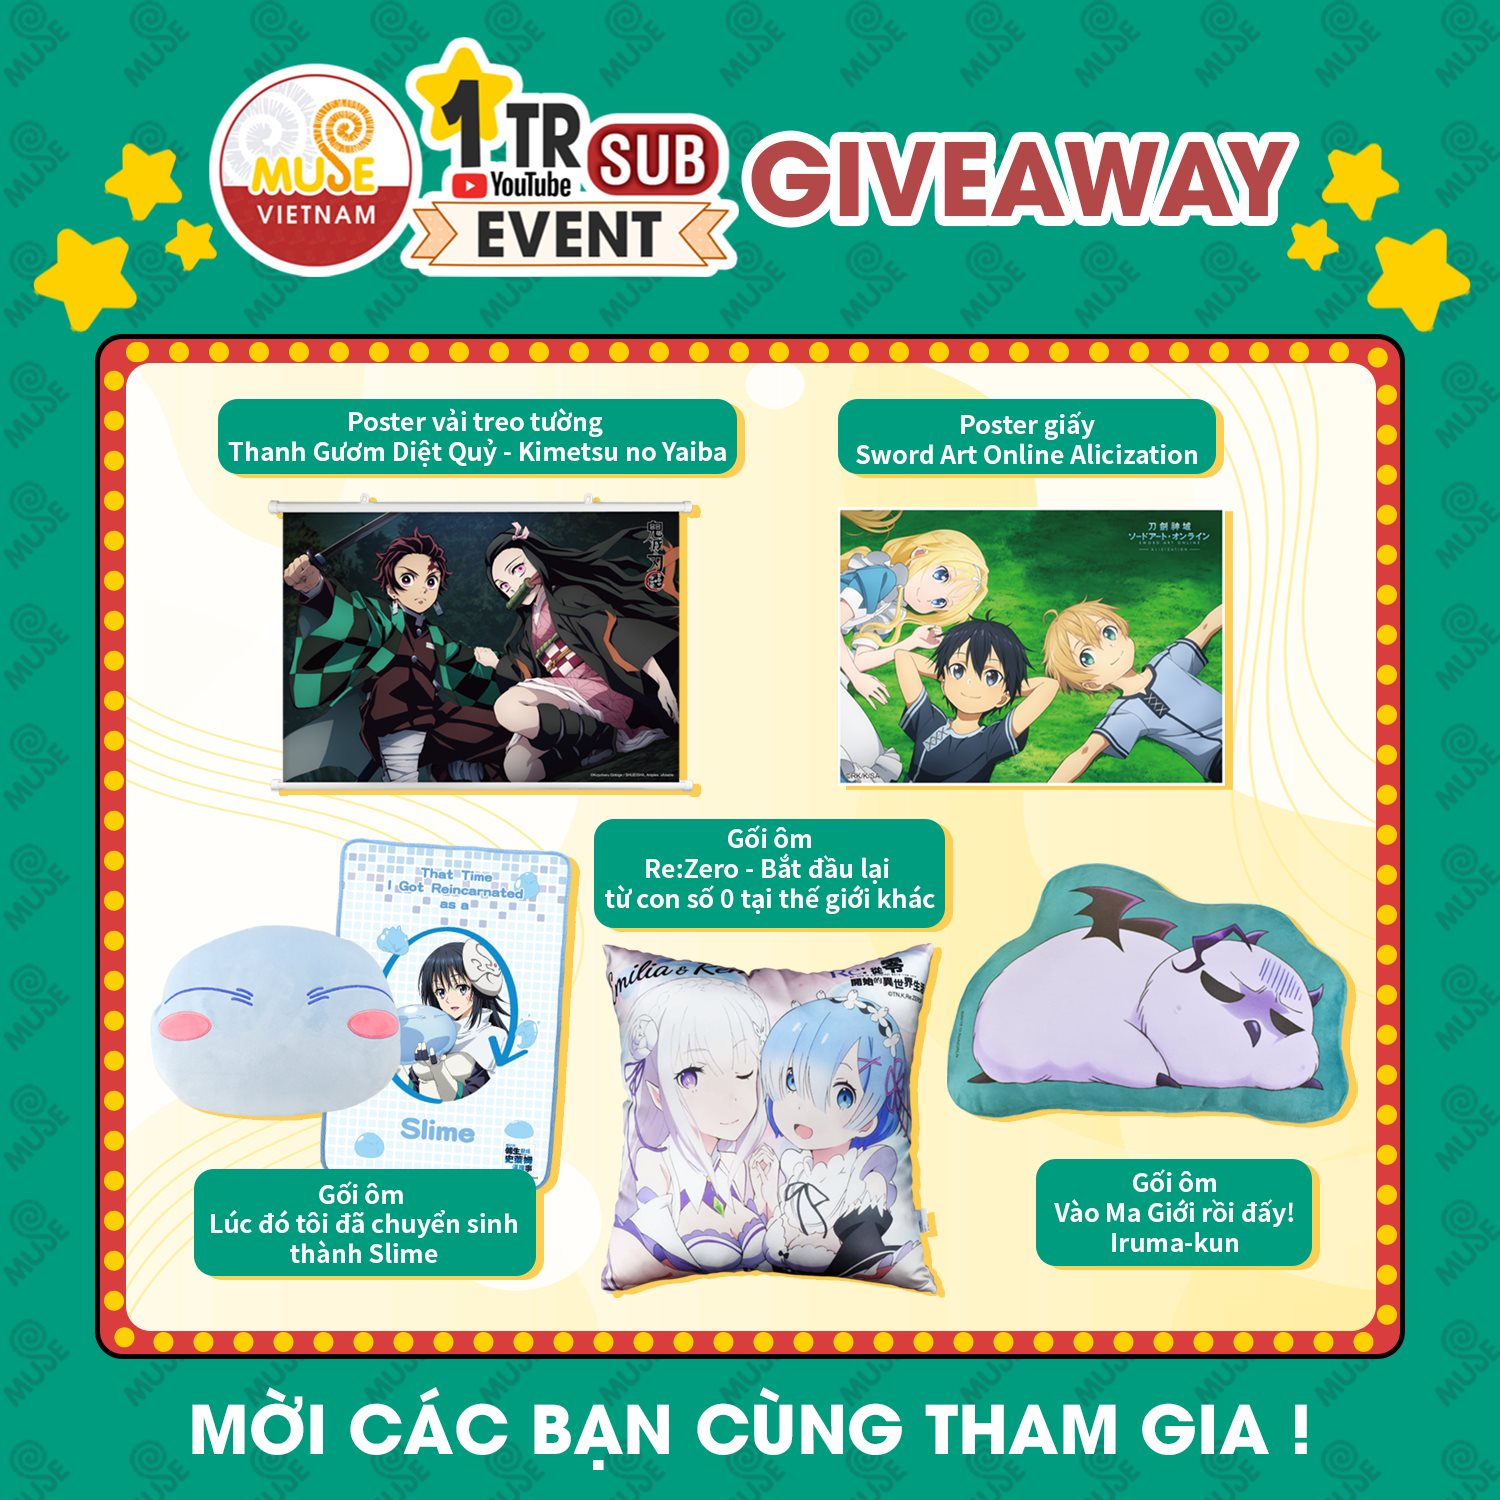
\includegraphics[width=\linewidth, height=0.5\linewidth]{content/background/image/muse.jpg}}
    \caption{Giveaway - Mừng kênh Muse Việt Nam đạt 1 triệu sub}
    \label{fig}
    \end{figure}
    \item Việc tiếp cận anime trở nên dễ dàng hơn thông qua các nền tảng trực tuyến như Netflix, YouTube, và Bilibili, giúp giới trẻ trải nghiệm nhiều tác phẩm đa dạng về thể loại.
    \begin{figure}[H]
    \centerline{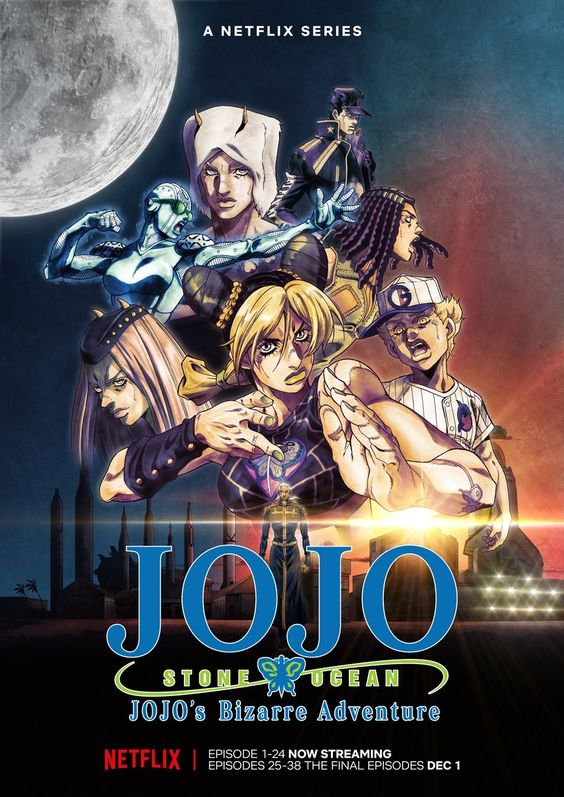
\includegraphics[width=\linewidth, height=0.5\linewidth]{content/background/image/netflix.jpg}}
    \caption{JoJo's Bizarre Adventure: Stone Ocean}
    \label{fig}
    \end{figure}
    \item Anime cũng trở thành công cụ quảng cáo hiệu quả, khi nhiều thương hiệu tận dụng hình ảnh này để thu hút khách hàng trẻ tuổi.
    \begin{figure}[H]
    \centerline{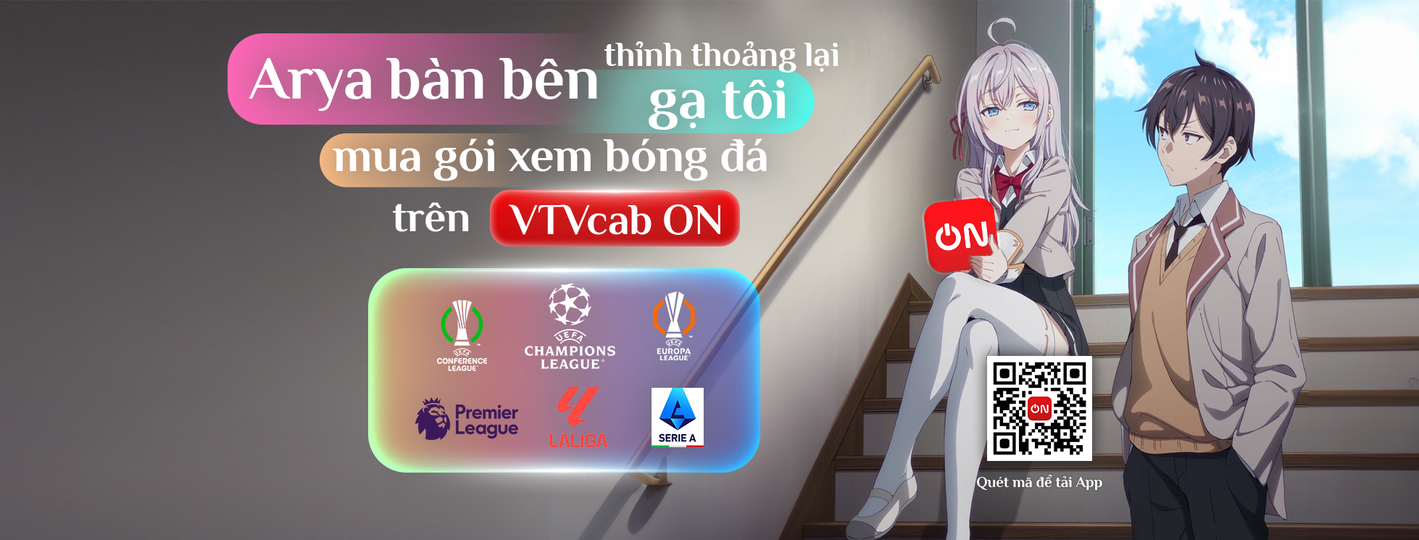
\includegraphics[width=0.8\linewidth, height=\linewidth]{content/background/image/vtvCab.png}}
    \caption{Chiến lược quảng cáo sử dụng hình ảnh anime kết hợp với nội dung bóng đá}
    \label{fig}
    \end{figure}
\end{itemize}

\headindent \textbf{Kết luận}: Anime đang trở thành một xu hướng văn hóa phổ biến và có tầm ảnh hưởng lớn tại Việt Nam, đặc biệt với giới trẻ. Sự phát triển của các cộng đồng yêu thích anime, sự đa dạng trong nguồn nội dung, và việc tích hợp anime vào các chiến lược quảng cáo đã giúp anime trở thành một phần không thể thiếu trong đời sống giải trí hiện đại. Điều này cho thấy tiềm năng phát triển mạnh mẽ của văn hóa anime tại Việt Nam trong tương lai.

\vspace{0.5cm}
\begin{figure}[H]
\centerline{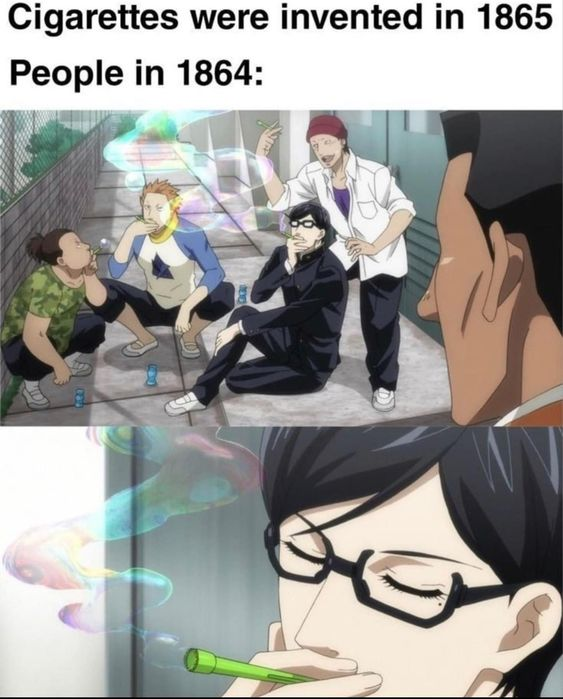
\includegraphics[width=\linewidth, height=0.6\linewidth]{content/background/image/cigarettes.jpg}}
\caption{Sakamoto Desu Ga Meme}
\label{fig}
\end{figure}
    
\pagebreak


